%%%%%%%%%%%%%%%%%%%%%%%%%%%%%%%%%%%%%%%%%%%%%%%%%%%%%%%%%%%%%%%%%%%%%%%%%%%%%%%
%     Problem setup
%%%%%%%%%%%%%%%%%%%%%%%%%%%%%%%%%%%%%%%%%%%%%%%%%%%%%%%%%%%%%%%%%%%%%%%%%%%%%%%

%\begin{frame}{Pulling hose problem}
%%
%  \begin{minipage}{0.55\textwidth}
%    \begin{center}
%      \movie[autostart,loop,continue]{
%        \includegraphics[width=\linewidth, height=\textheight, keepaspectratio]
%        {hose_xp/withoutwalkingtask.png}
%      }
%      {./videos/wihtoutwalkingtask.mpg}
%    \end{center}
%  \end{minipage}  \hfill
%%
%\only<1>{
%  \begin{minipage}{0.42\textwidth}
%    \textbf{\color{txtcolor2} Setup :}
%    \begin{itemize}
%      \item HRP-2 humanoid robot
%      \item rigid, \emph{empty} fire hoze
%      \item motion capture system
%    \end{itemize}
%  \end{minipage}
%}
%%
%\only<2>{
%  \begin{minipage}{0.41\textwidth}
%    \textbf{\color{txtcolor2} Major technical issues while}
%    \begin{itemize}
%%
%    \item \textbf{\color{txtcolor2} pulling :}
%    \begin{itemize}
%      \item Important drift
%      \item Robot less balanced
%    \end{itemize}
%%    
%    \item \textbf{\color{txtcolor2} picking :}
%      \begin{itemize}
%        \item Self-collision
%        \item Joint limit
%        \item Balance
%      \end{itemize}
%%    
%    \end{itemize}
%  \end{minipage}
%}
%%
%\only<3>{
%  \begin{minipage}{0.39\textwidth}
%    \textbf{\color{txtcolor2} Objectives :}
%    \begin{itemize}
%      \item Pick up a rigid fire hose
%      \item Pull it toward a desired position
%    \end{itemize}
%    \vspace*{0.7cm}
%  \end{minipage}
%}
%
%\end{frame}
 
\begin{frame}{Pulling hose problem}
  \vspace*{-0.5cm}
  \begin{center}
    \movie[autostart,loop,continue]{
      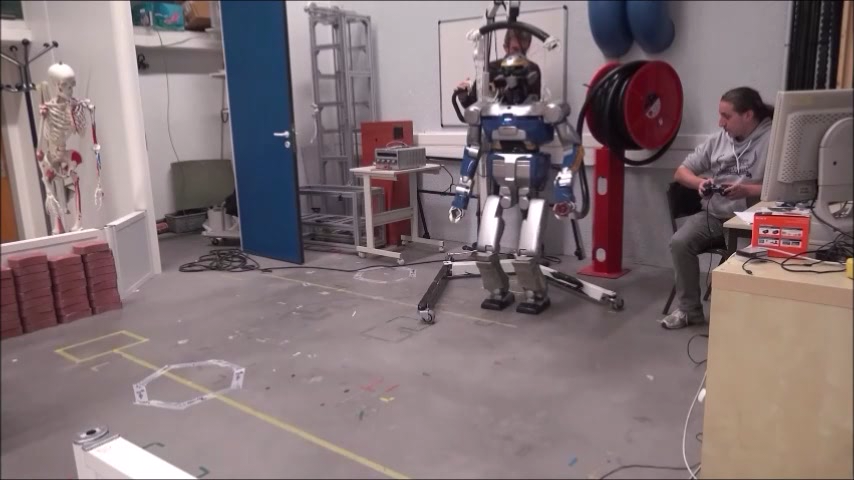
\includegraphics[height=0.5\textheight, keepaspectratio]
      {hose_xp/withoutwalkingtask.png}
    }
    {./videos/wihtoutwalkingtask.mpg}
  \end{center} 
  \begin{itemize}
    \item Observation : important drift, robot less balanced
    \item Hypothesis :
    \begin{itemize}
      \item simple controller is enough to correct the drift
      \item admittance control should reject the perturbation 
    \end{itemize}
  \end{itemize}
\end{frame} 
 
%%%%%%%%%%%%%%%%%%%%%%%%%%%%%%%%%%%%%%%%%%%%%%%%%%%%%%%%%%%%%%%%%%%%%%%%%%%%%%%%%%%%%%%%
%
%\begin{frame}{Pick Up Motion}
%  \vspace*{0.6cm}
%  \begin{center}
%    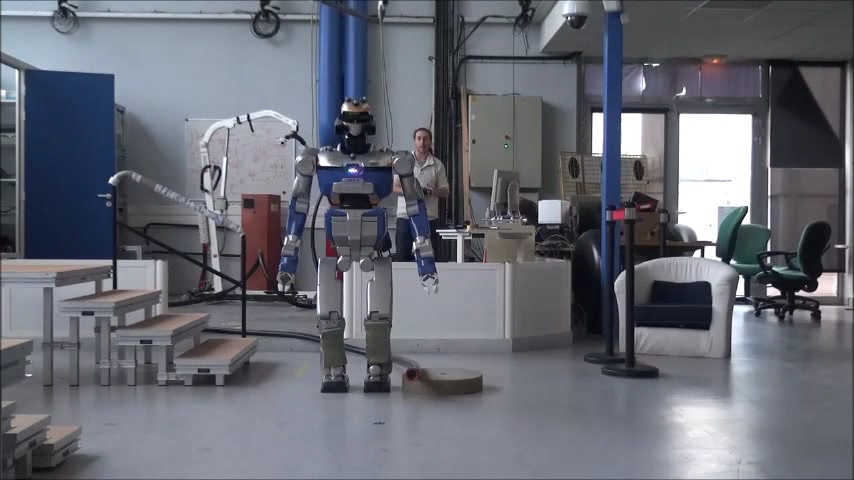
\includegraphics[height = 4.0cm]{hose_xp/pickup.png}
%  \end{center}
%%
%  \vspace*{-1ex}
%  \textbf{\color{txtcolor2} Planning constraint using HPP :}\\
%%  
%  \begin{minipage}{0.45\textwidth}
%    \begin{itemize}
%      \item Static Balance
%      \item Feet flat on the floor
%      \item Left wrist position
%    \end{itemize}
%  \end{minipage}
%%
%  \begin{minipage}{0.50\textwidth}
%    \begin{itemize}
%      \item Robot facing forward
%      \item Close from half-sitting position
%    \end{itemize}
%    \vspace*{0.4cm}    
%  \end{minipage}
%%
%  \begin{center}
%    \small{\color{txtcolor3}\url{https://humanoid-path-planner.github.io/hpp-doc}}
%  \end{center}
%%
%\end{frame}
%
%%%%%%%%%%%%%%%%%%%%%%%%%%%%%%%%%%%%%%%%%%%%%%%%%%%%%%%%%%%%%%%%%%%%%%%%%%%%%%%%%%%%%%%%
%
%\begin{frame}{Walking task}
%  \vspace*{0.2cm}
%  \begin{center}
%    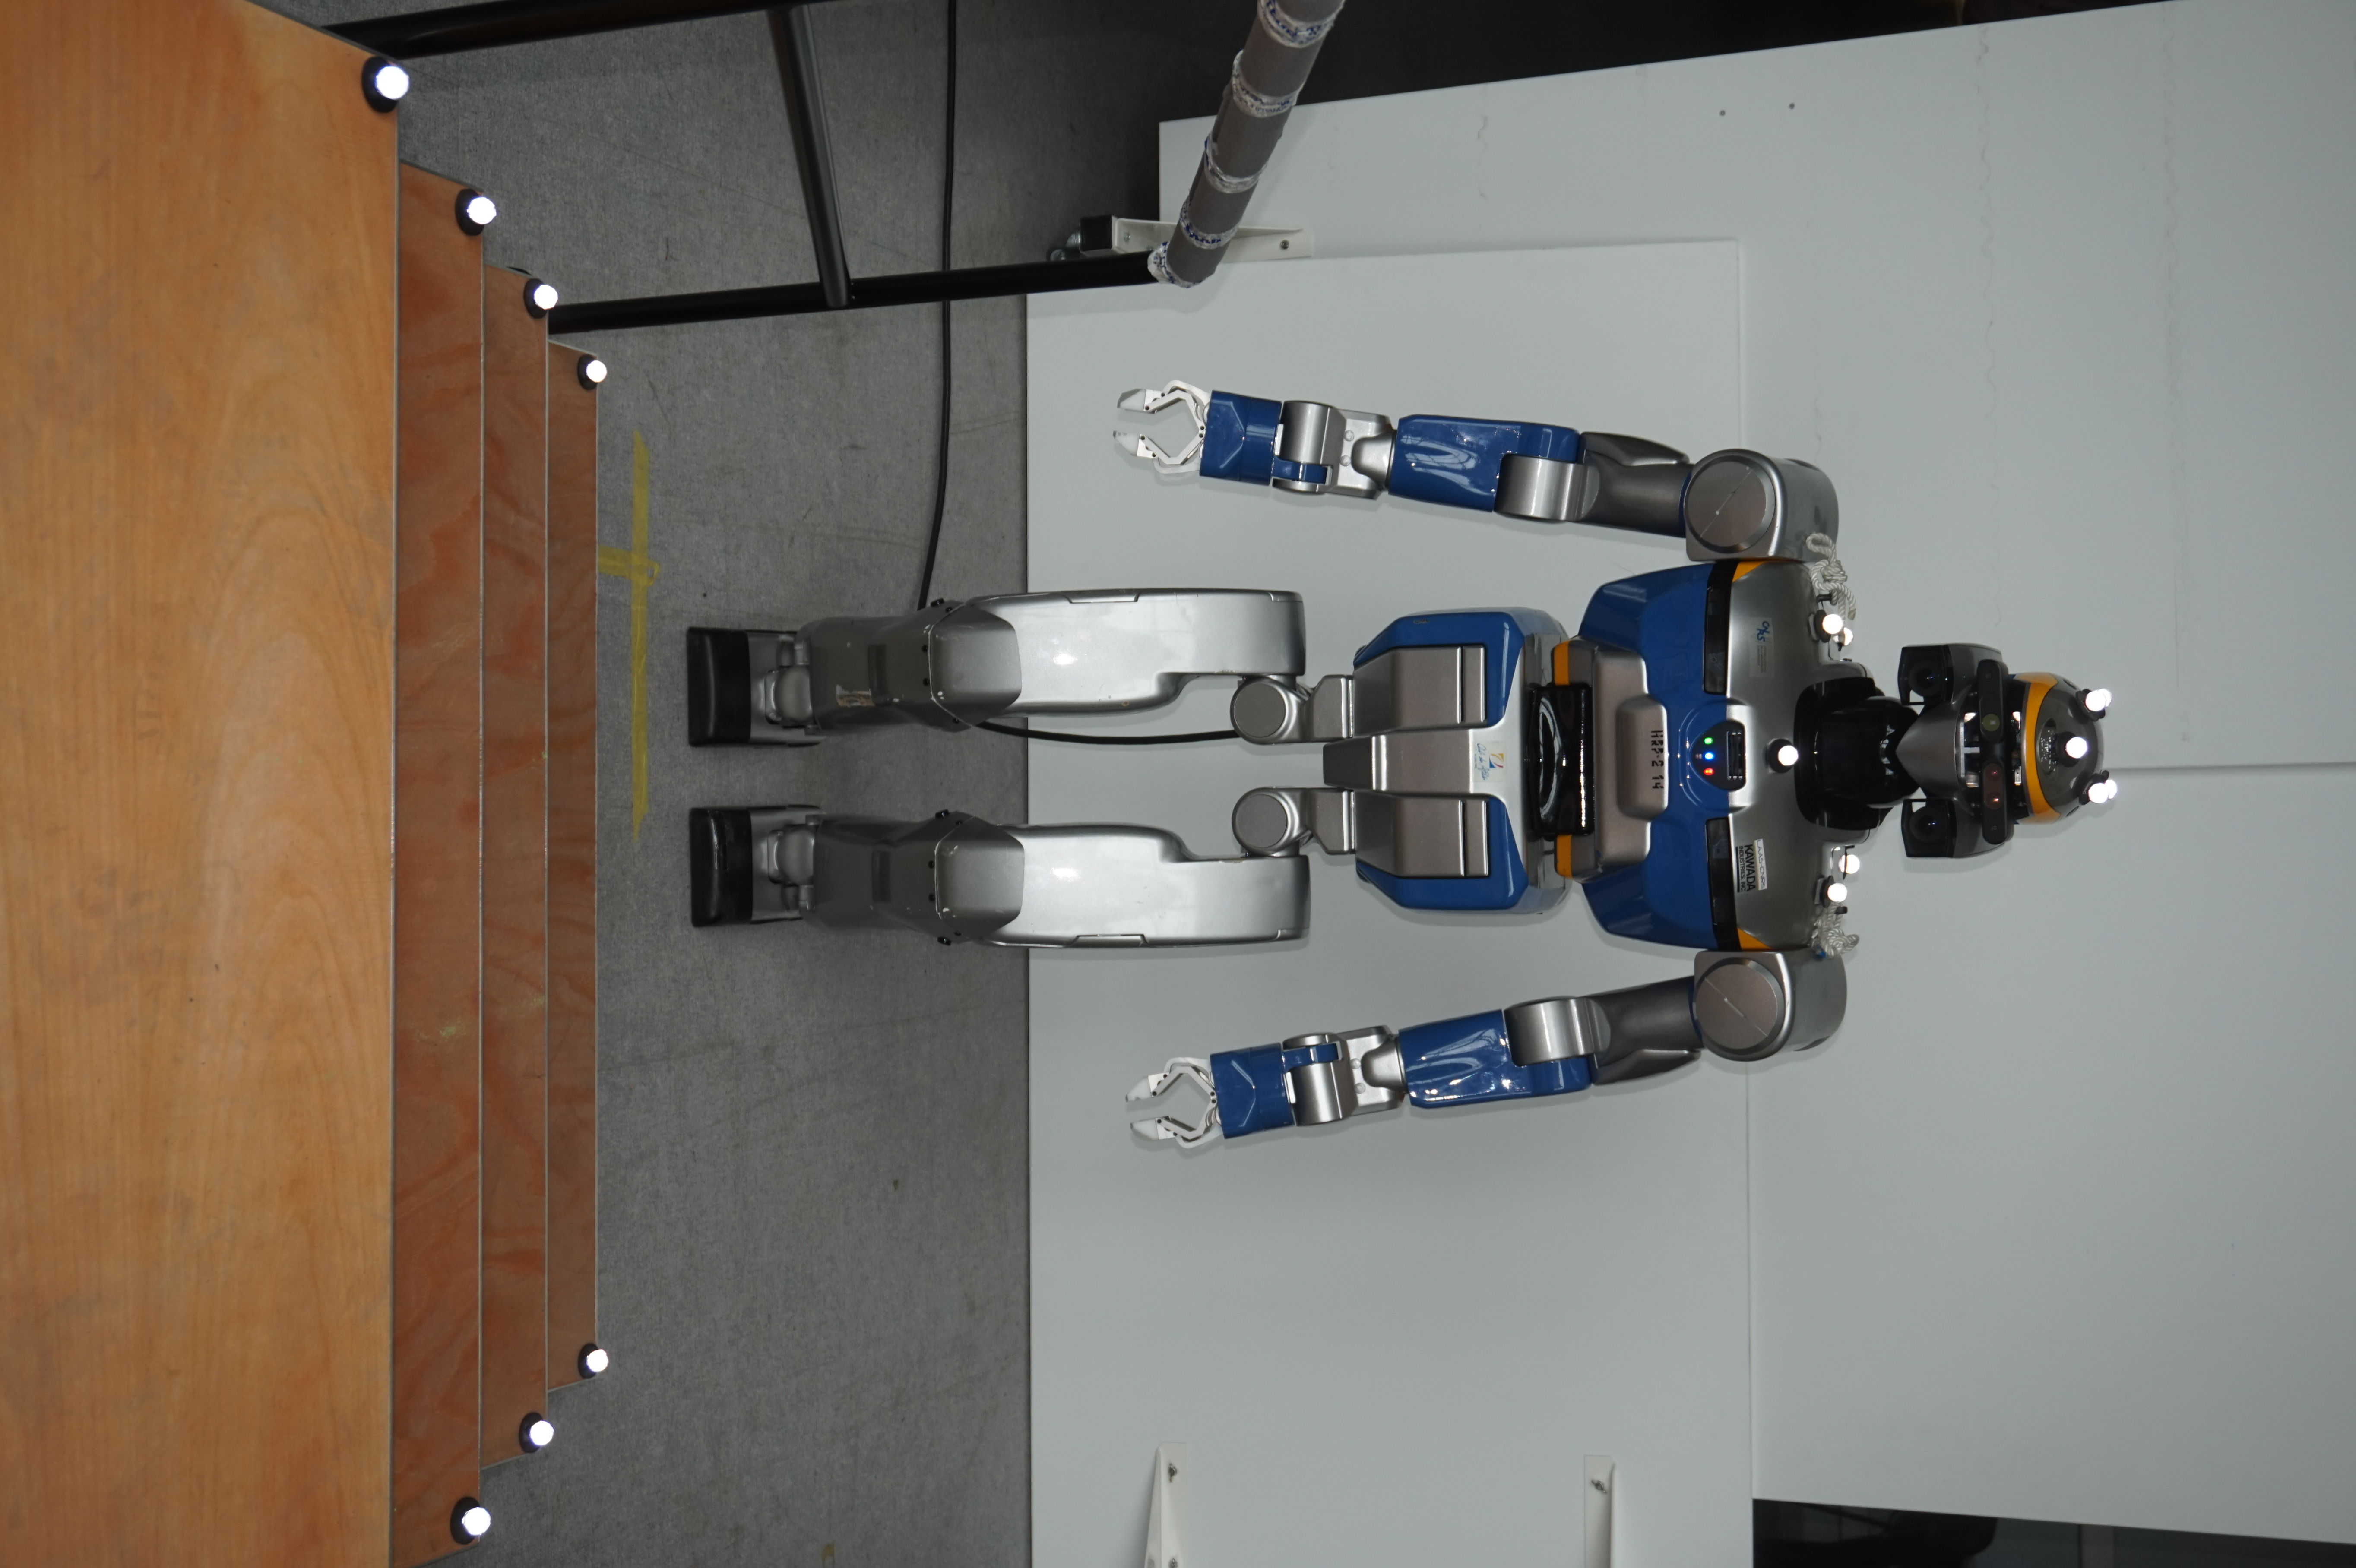
\includegraphics[angle=90, height=0.25\paperheight]{./DSC00610.JPG}
%    \hspace*{1.5cm}
%    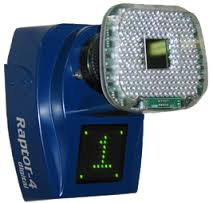
\includegraphics[height=0.25\paperheight]{./camera_raptor.jpeg}
%  \end{center}
%
%  \tikzstyle{na} = [baseline=-.5ex]
%  \begin{itemize}
%    \item adaptive gains
%      \tikz[na] \node[coordinate] (l) {};
%    \item referenced velocity 
%      \tikz[na] \node[coordinate] (vr) {};
%  \end{itemize}
%%
%%  \vspace*{-0.5cm}
%  \begin{align*}
%    \;\;\;\;\;\;\;\;\;\;\;\;\;\;\;\;\;\;\;\;\;\;\;\;\;
%    \tikz[baseline]{
%      \node[fill=txtcolor1,anchor=base] (v)
%      { $ \mathbf{v}^{\mathrm{ref}} $ };
%    }
%    = - \tikz[baseline]{
%      \node[fill=txtcolor2,anchor=base] (l1)
%      {$\lambda$};
%    } \;
%    \tikz[baseline]{
%      \node[fill=txtcolor3,anchor=base] (e1)
%      {$ \mathbf{e}_{w} $};
%    } - 
%    \tikz[baseline]{
%      \node[fill=txtcolor2,anchor=base] (l2)
%      {$ \mathbf{\Lambda} $};
%    }
%    \int \tikz[baseline]{
%      \node[fill=txtcolor3,anchor=base] (e2)
%      {$ \mathbf{e}_{w} $};
%    } dt
%  \end{align*}
%
%  \begin{itemize}
%    \item $ 
%     \tikz[baseline]{
%      \node[fill=txtcolor3,anchor=base] (e3)
%      {$ \mathbf{e}_{w} $};
%    }
%     = 
%     \begin{bmatrix}
%       x_{chest} & y_{chest} & \theta_{chest}
%     \end{bmatrix}^T
%     -$\tikz[na] \node[coordinate] (e) {};\\
%     $
%     \begin{bmatrix}
%       x^{des}_{chest} & y^{des}_{chest} & \theta^{des}_{chest}
%     \end{bmatrix}^T $
%  \end{itemize}
%%
%% Now it's time to draw some edges between the global nodes. Note that we
%% have to apply the 'overlay' style.
%  \begin{tikzpicture}[overlay]
%    \path[->,line width=0.5mm, txtcolor1] (vr) edge [bend left] (v);
%    \path[->,line width=0.5mm, txtcolor3] (e) edge [bend right] (e1);
%    \path[->,line width=0.5mm, txtcolor3] (e) edge [bend right] (e2);
%    \path[->,line width=0.5mm, txtcolor2] (l) edge [bend left] (l1);
%    \path[->,line width=0.5mm, txtcolor2] (l) edge [bend left] (l2);
%  \end{tikzpicture}
%%  
%\end{frame}
%
%
%%%%%%%%%%%%%%%%%%%%%%%%%%%%%%%%%%%%%%%%%%%%%%%%%%%%%%%%%%%%%%%%%%%%%%%%%%%%%%%%%%%%%%%%
%
%\begin{frame}{Hybrid controller}
%  \tikzstyle{na} = [baseline=-0.5ex]
%  \begin{center}
%    \includegraphics[width=0.45\textwidth]
%    {hose_xp/force_Z_feet_withoutController_zoomEnd.pdf}\hfill
%    \includegraphics[width=0.45\textwidth]
%    {hose_xp/force_Z_feet_withController_zoomEnd.pdf}\\
%    \textbf{\color{txtcolor1} without the controller}
%    \tikz[na] \node[coordinate] (without) {};
%    \hfill
%    \tikz[na] \node[coordinate] (with) {};    
%    \textbf{\color{txtcolor1} with the controller}
%    \hfill \hfill
%  \end{center}  
%  
%  \begin{tikzpicture}[overlay]
%    \path[->,line width=0.5mm, txtcolor1] (without) edge (with);
%  \end{tikzpicture}
%  \vspace*{-1cm}
%
%%  \tikzstyle{na} = [baseline=-0.5ex]
%%   \tikz[na] \node[coordinate] (nfpull) {};
%%  desired force \tikz[na] \node[coordinate] (nfd) {};
%%  external force \tikz[na] \node[coordinate] (nflw) {};
%%  left wrist velocity and acceleration \tikz[na] \node[coordinate] (nav) {};
%
%%  
%%  \begin{itemize}
%%    \item pulling force
%%      \tikz[na] \node[coordinate] (nfpull) {};
%%    \item desired force
%%      \tikz[na] \node[coordinate] (nfd) {};
%%    \item wrist measured \\external force 
%%      \tikz[na] \node[coordinate] (nflw) {};
%%  \end{itemize}
%%
%\begin{small}
%  \begin{align*}
%    m & \tikz[baseline]{
%      \node[fill=txtcolor1,anchor=base] (a)
%      { $ \ddot{\bf lw}^{x} $ };
%    }
%   + c \tikz[baseline]{
%      \node[fill=txtcolor1,anchor=base] (v)
%      {$ \dot{\bf lw}^{x} $};
%    } = 
%    \tikz[baseline]{
%      \node[fill=txtcolor4,anchor=base] (flw)
%      {$ {\bf f}_{lw}^{x} $};
%    } + 
%    \tikz[baseline]{
%      \node[fill=txtcolor2,anchor=base] (fd)
%      {$ {\bf f}_{d}^{x} $};
%    } + 
%    \tikz[baseline]{
%      \node[fill=txtcolor3,anchor=base] (fpull)
%      {$ {\bf f}_{pull}^{x} $};
%    }
%    %
%    \\
%    %
%    m & \tikz[baseline]{
%      \node[fill=txtcolor1,anchor=base] (a)
%      { $ \ddot{\bf lw}^{z} $ };
%    }
%   + c \tikz[baseline]{
%      \node[fill=txtcolor1,anchor=base] (v)
%      {$ \dot{\bf lw}^{z} $};
%    } = 
%    \tikz[baseline]{
%      \node[fill=txtcolor4,anchor=base] (flw)
%      {$ {\bf f}_{lw}^{z} $};
%    } + 
%    \tikz[baseline]{
%      \node[fill=txtcolor2,anchor=base] (fd)
%      {$ {\bf f}_{d}^{z} $};
%    } + 
%    \tikz[baseline]{
%      \node[fill=txtcolor3,anchor=base] (fpull)
%      {$ {\bf f}_{pull}^{z} $};
%    }
%    %
%    \\
%    %
%    &\tikz[baseline]{
%      \node[fill=txtcolor1,anchor=base] (a)
%      { $ {\bf lw}^{y} $ };
%    } = {\bf waist}^{y} + \text{offset}
%  \end{align*}
%\end{small}
%%  \begin{itemize}
%%    \item left wrist velocity\\
%%    and acceleration \tikz[na] \node[coordinate] (nav) {};
%%  \end{itemize}
%
%% Now it's time to draw some edges between the global nodes. Note that we
%% have to apply the 'overlay' style.
%%  \begin{tikzpicture}[overlay]
%%    \path[->,line width=0.5mm, txtcolor1]  (nav) edge [bend right] (a);
%%    \path[->,line width=0.5mm, txtcolor1]  (nav) edge [bend right] (v);
%%    \path[->,line width=0.5mm, txtcolor4]   (nflw) edge [bend left] (flw);
%%    \path[->,line width=0.5mm, txtcolor2](nfd) edge [bend left] (fd);
%%    \path[->,line width=0.5mm, txtcolor3]   (nfpull) edge [bend left] (fpull);
%%  \end{tikzpicture}
%  
%\end{frame}


%%%%%%%%%%%%%%%%%%%%%%%%%%%%%%%%%%%%%%%%%%%%%%%%%%%%%%%%%%%%%%%%%%%%%%%%%%%%%%%%%%%%%%%

\begin{frame}{3 combined controllers}
%
  \begin{minipage}{0.3\textwidth}
    \begin{center}
      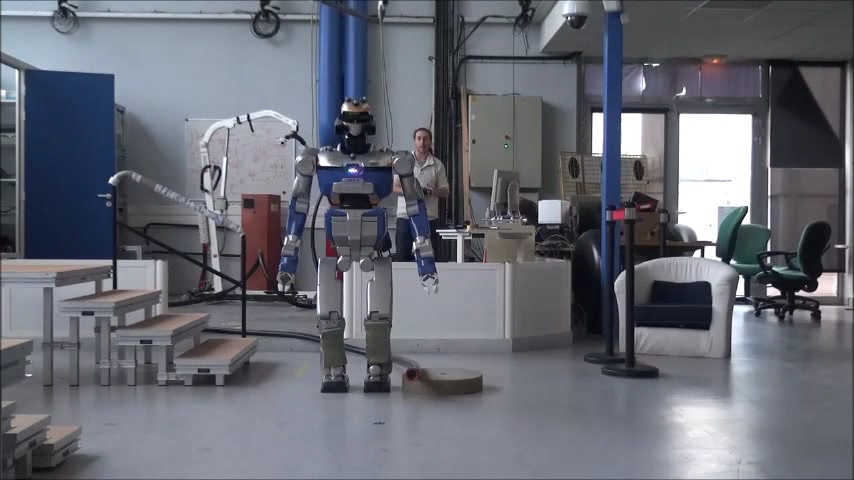
\includegraphics[trim={7.0cm 2.0cm 10.5cm 2.0cm}, clip, height=0.30\textheight]
      {hose_xp/pickup.png}
      %trim={<left> <lower> <right> <upper>}
    \end{center}
  \end{minipage}
%
{\color{txtcolor2}\vrule}
  \begin{minipage}{0.3\textwidth}
    \begin{center}
      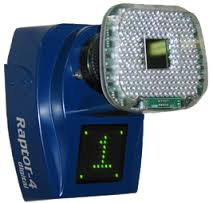
\includegraphics[height=0.20\textheight]{./camera_raptor.jpeg}
    \end{center}
  \end{minipage}
%
{\color{txtcolor2}\vrule}    
  \begin{minipage}{0.3\textwidth}
    \begin{center}
      {\scriptsize Without the controller}
      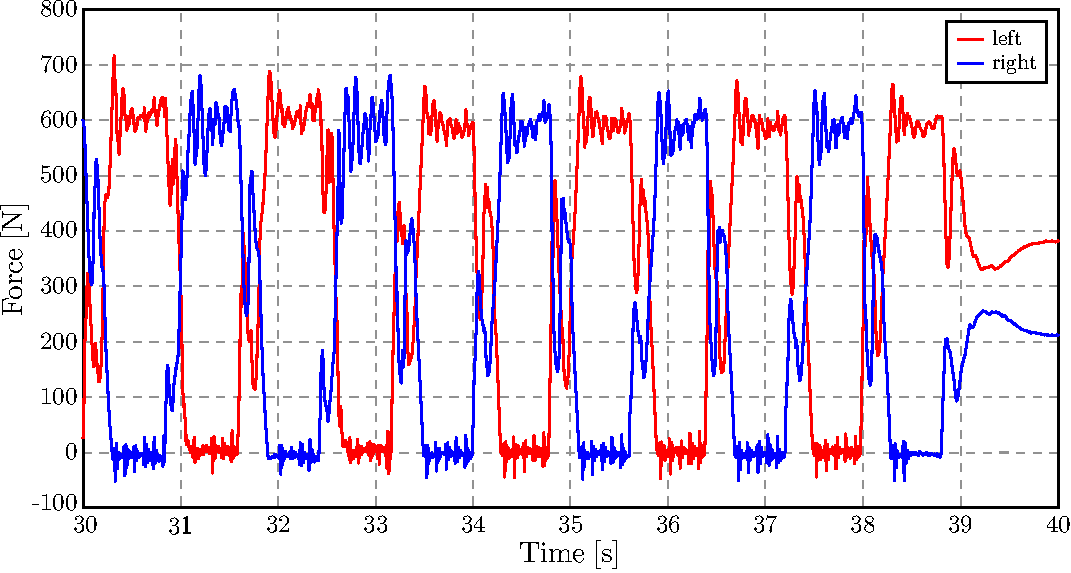
\includegraphics[trim={5.0cm 1.5cm 7.0cm 1.0cm}, clip, width=\textwidth , height=0.15\textheight]
      {hose_xp/force_Z_feet_withoutController_zoomEnd.pdf}\\[1.ex]
      {\scriptsize With the controller}
      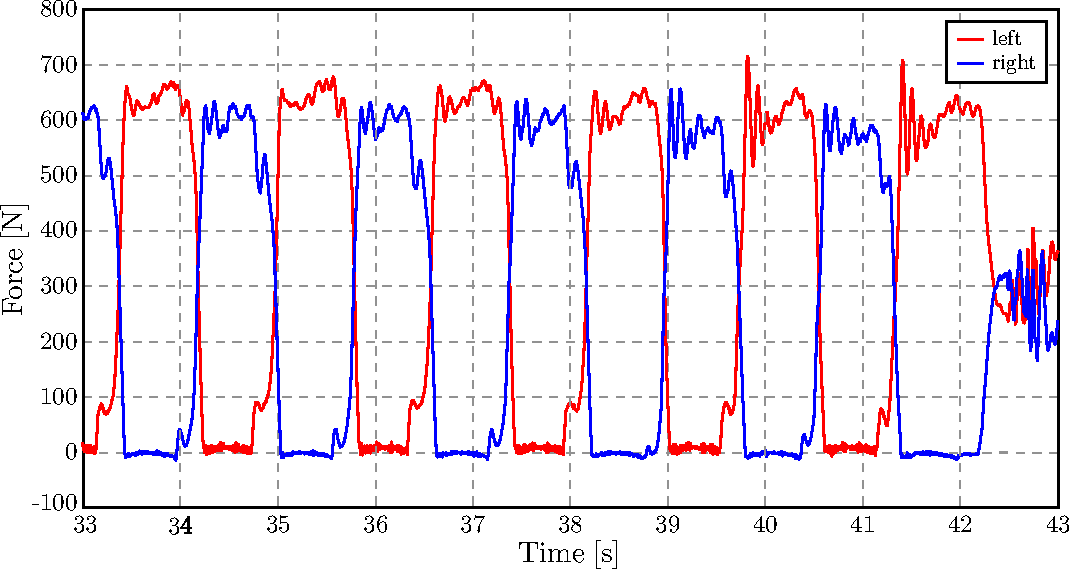
\includegraphics[trim={5.0cm 1.5cm 7.0cm 1.0cm}, clip, width=\textwidth , height=0.15\textheight]
      {hose_xp/force_Z_feet_withController_zoomEnd.pdf}\\
      %trim={<left> <lower> <right> <upper>}
      {\scriptsize {\color{blue}left}/{\color{red}right} foot $z$ forces}
      \end{center}
  \end{minipage}\\[-1ex]
%   
  \begin{minipage}{0.3\textwidth}
    \vspace*{-1cm}
    Planning:
    \begin{itemize}
      \item Static Balance
      \item Feet flat
      \item (Self-)Collisions
    \end{itemize}
  \end{minipage}
%
{\color{txtcolor2}\vrule}
  \begin{minipage}{0.3\textwidth}
    \vspace*{-0.2cm}
    Position Control :
    \begin{itemize}
      \item Reactive Walking
      \item Localization via motion capture
      \item {\footnotesize Perturbation rejection}\textbf{{\scriptsize (in progress)}}
    \end{itemize}
  \end{minipage}
%
{\color{txtcolor2}\vrule}
  \begin{minipage}{0.3\textwidth}
    \vspace*{-0.5cm}
    \begin{itemize}
    \item Hybrid Control on the left gripper
    \end{itemize}
  \end{minipage}
%
\end{frame}

%%%%%%%%%%%%%%%%%%%%%%%%%%%%%%%%%%%%%%%%%%%%%%%%%%%%%%%%%%%%%%%%%%%%%%%%%%%%%%%%%%%%%%%
%
%\begin{frame}{Full controller}
%  \scalebox{0.7}{%!TEX root = ../../14-icra-RealTimeNMPC.tex

\tikzstyle{block} = [draw, fill=blue!20, rectangle,
    minimum height=2em, minimum width=5em, align=center]
\tikzstyle{sum} = [draw, fill=blue!20, circle, node distance=1cm]
\tikzstyle{input} = [coordinate]
\tikzstyle{output} = [coordinate]
\tikzstyle{pinstyle} = [pin edge={to-,thin,black}]

% The block diagram code is probably more verbose than necessary
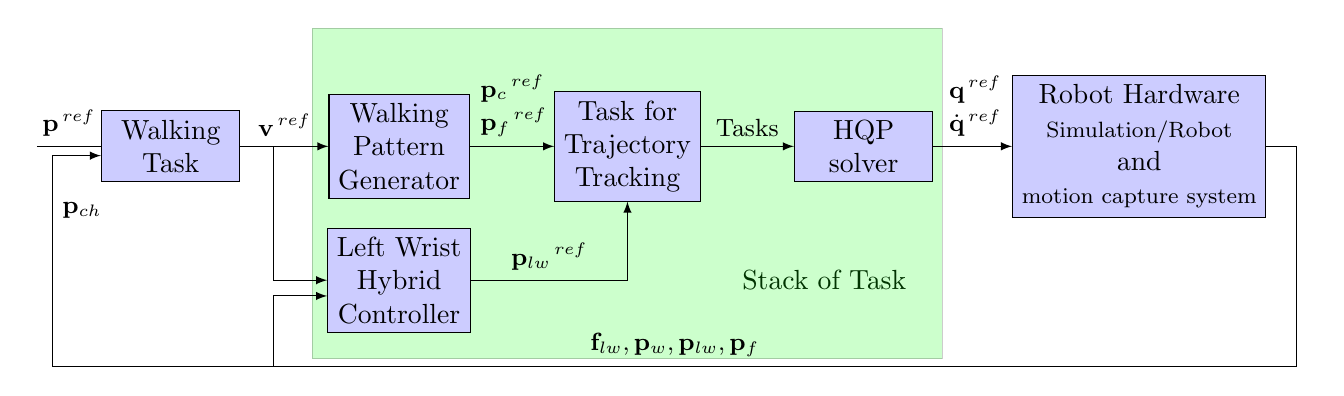
\begin{tikzpicture}[auto, node distance=2cm,>=latex]

    % We start by placing the blocks
    \node [input]  at (0.0, 0.0) (input)  {};
    \node [input]  at (3, 0.0) (velocity) {};
    \node [input]  at (0.2, -2.8) (feedback)  {};
    \node [input]  at (16, -2.8) (feedback2)  {};
    \node []    at ( 0.0, 0.0) (sumin)  {};
    %\node [output]    at ( 15, 0.0) (sumout) {};
    \draw [fill=green,opacity=.2,text opacity=1] (3.5,1.5) rectangle (11.5,-2.7);
    \node at(10,-1.7) {\textcolor{green!20!black!100}{Stack of Task}};

    \node [block] at (4.6,-1.7) (lwc) {
        Left Wrist\\
        Hybrid\\
        Controller        
    };

    \node [block] at (1.7,0.0) (walking) {
        Walking \\
        Task    
    };

    \node [block] at (4.6,0) (wpg) {
        Walking\\
        Pattern\\
        Generator
    };
%    \node [block] at (4.2,0) (dyn) {
%        Dynamic\\
%        Filter
%    };
    \node [block] at (7.5,0) (ttt) {
        Task for\\
        Trajectory\\
        Tracking
    };
    
    \node [block] at (10.5,0) (qp) {
        HQP\\
        solver
    };

    \node [block] at (14.0, 0) (system) {
    		Robot Hardware\\
    		{\footnotesize Simulation/Robot}\\
    		and\\
    		{\footnotesize motion capture system}
    	};

    % PATHS
    	% Forward chaine
    \draw [draw,-] (input) -- node {\small ${\mathbf{p}}^{\,{\text {ref}}}$} (walking);
    
    \draw [draw,->] (walking) -- node {\small ${\mathbf v}^{\,{\text{ref}}}$} (wpg);
%    \draw [draw,- ] (walking) -- node {} (velocity);
    \draw [draw,->] (velocity) |- node {} (lwc);
%    \draw [->] (wpg) -- node {\small $c^{ref},f^{ref}$} (dyn);
%    \draw [->] (dyn) -- node {\small $\tilde{c}^{\,ref},f^{ref}$} (sot);
    \draw [->] (wpg) -- node [text width=0.8cm]{\small ${\mathbf{p}_c}^{\,{\text {ref}}}$ ${\mathbf{p}_f}^{\,{\text {ref}}}$} (ttt);
    \draw [->] (ttt) -- node [text width=0.8cm]{
    \small Tasks
    } (qp);
    \draw [->] (qp) -- node [text width=0.6cm]{\small ${\mathbf q}^{\,{\text{ref}}}$ $\dot{{\mathbf q}}^{\,{\text{ref}}}$} (system);
    
    \draw [->] (lwc) -| node [near start, above]{\small ${\mathbf{p}_{lw}}^{\,{\text {ref}}}$} (ttt);
    %\draw [->] (system) -- node {} (sumout);

    % Feedback chaine
%    \draw [- ] (dyn)      -| node {} (feedback);
%    \draw [->] (feedback) -| node {} (wpg);
    
    \draw [- ] (system.east)    -| node {} (feedback2);
    \draw [- ] (feedback2)  -- node [above]{\small $\mathbf{f}_{lw},\mathbf{p}_{w},\mathbf{p}_{lw},\mathbf{p}_{f}$} (feedback);
    \draw [->] (3.0,-2.8) |- node [near start, above]{} ([yshift=-0.2cm]lwc.west);
    \draw [->] (feedback) |- node [below=0.7cm, right]{\small $\mathbf{p}_{ch}$} ([yshift=-0.2cm]walking);

%    \draw [->] (dyn) -| node[above right] {\small $\hat{c}^{\,x,y,\theta}$, $\hat{f}^{\,\,x,y,\theta}$} (wpg);
\end{tikzpicture}
} \\
%%
%
%%  \textbf{\color{blue}Full feedback scheme}
%%
%\end{frame}

\begin{frame}{Complete motion}
  \begin{center}
    \movie[autostart,loop]{
    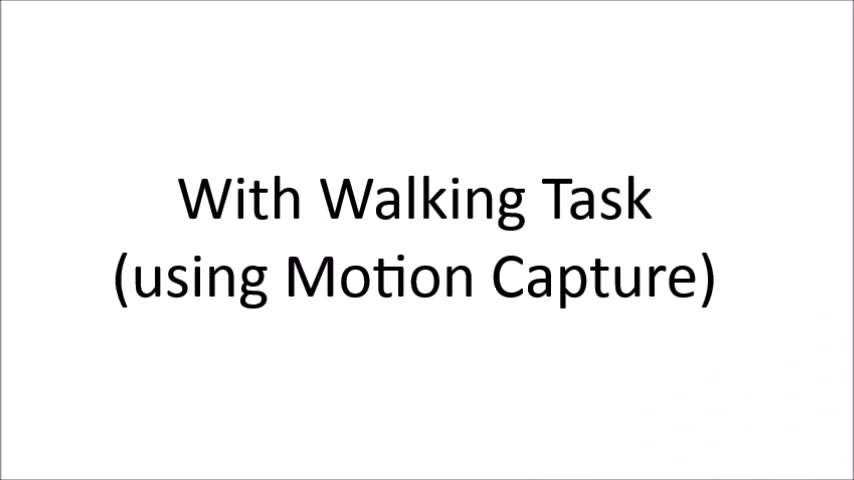
\includegraphics[width=0.8\linewidth, height=\textheight, keepaspectratio]
    {hose_xp/wholemotion.png}    
    }  
    {./videos/wholemotion.mpg}
  \end{center}
  \vspace*{-0.5cm}
  \blfootnote{Ramirez-Alpizar, \textbf{Naveau} et al. Humanoids 2016}
\end{frame}